\section{Facit}
%%
%%
\setcounter{opgave}{0}

%%
%%
\begin{opgave}{Hastighed og postion}
	\begin{figure}[h!]
		\centering
		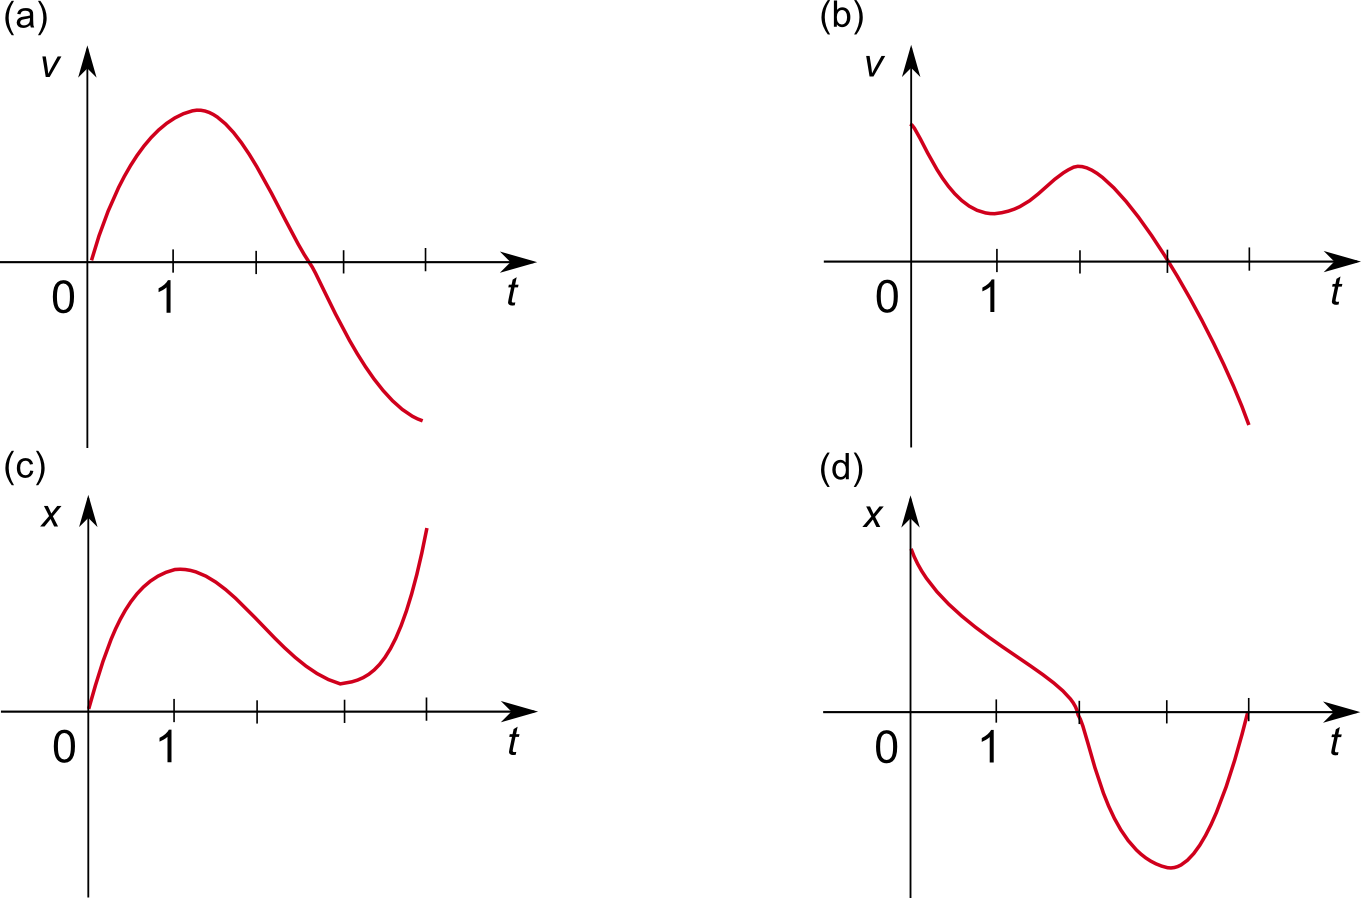
\includegraphics[width=0.47\textwidth]{opg/figurer/vx_grafer.png}
		\caption{Hastighed og position som funktion af tiden.}
		\label{fig:vx_grafer}
	\end{figure}
	\opg Figur \ref{fig:vx_grafer} (a) og (b) viser hastigheden af to objekter som funktion af tiden i sekunder. Hvornår sætter de to objekter hastigheden op, og hvornår sætter de hastigheden ned? Forklar dit svar.
	
	De to objekter sætter hastigheden op når accelerationen er positiv, d.v.s. at hastighedsgrafen er stigende.
	For (a) er det inden toppunktet lidt efter $t=1$.
	For (b) stiger hastigheden imellem $t=1$ og $t=2$.
	\opg Figur \ref{fig:vx_grafer} (c) og (d) viser positionen af to objekter $x$ som funktion af tiden i sekunder. Hvornår sætter de to objekter hastigheden op, og hvornår sætter de hastigheden ned? Forklar dit svar.
	
	De to objekter sætter hastigheden op når accelerationen er positiv, d.v.s. at krumningen er positiv. Her bruges smiley reglen.
	
	For (c) er krumningen negativ fra $t=0$ til $t=2$, og derefter positiv.
	For (d) er krumningen positiv over alt undtagen et lille stykke imellem $t=1$ og $t=2$.
\end{opgave}
%%
\begin{opgave}{Afledede og dobbeltafledede}{1}
Find den afledede og dobbeltafledede med hensyn til $x$ for følgende funktioner:
\opg $f(x) = x^3$:
    \begin{align*}
        \dv{f}{x}&=3x^2 \: , \\
        \dv[2]{f}{x}&=6x \: .
    \end{align*}
\opg $f(x) = x^2 + 4x$:
    \begin{align*}
        \dv{f}{x}&=2x+4 \: ,\\
        \dv[2]{f}{x}&=2 \: .
    \end{align*}
\opg $f(x) = \frac{1}{x} + \frac{1}{x^2}$:
    \begin{align*}
        \dv{f}{x}&=-\frac{1}{x^2}-\frac{2}{x^3} \: , \\
        \dv[2]{f}{x}&=\frac{2}{x^3}+\frac{3}{x^4} \: .
    \end{align*}
\opg $f(x) = \cos(x)$:
    \begin{align*}
        \dv{f}{x}&=-\sin(x) \: , \\
        \dv[2]{f}{x}&= -\cos(x) \: .
    \end{align*}
\opg $f(x) = \ln(x)$:
    \begin{align*}
        \dv{f}{x}&=\frac{1}{x} \: , \\
        \dv[2]{f}{x}&=\frac{-1}{x^2} \: .
    \end{align*}

Til de sidste to delopgaver skal vi bruge produktregelen, der siger at den afledte af en funktion er: $\dv{}{x}\big(f(x)g(x)\big)=\dv{f}{x}g(x)+f(x)\dv{g}{x}$.
\opg $f(x) = x \sin(x)$:
    \begin{align*}
        \dv{f}{x}&=\sin(x)+x\cos(x) \: , \\
        \dv[2]{f}{x}&=2\cos(x)-x\sin(x) \: .
    \end{align*}
\opg $f(x) = \frac{1}{x} \ln(x)$:
    \begin{align*}
        \dv{f}{x}&=\frac{1}{x}\cdot \frac{1}{x}-\frac{1}{x^2}\cdot \ln(x)=\frac{1-\ln(x)}{x^2} \: , \\
        \dv[2]{f}{x}&=\frac{-1}{x^2}+\frac{2\ln(x)}{x^3}-\frac{1}{x^3}=\frac{2\ln(x)-x-1}{x^3} \: .
    \end{align*}

Her kunne man også have brugt kvotient regelen.
\end{opgave}
%%
\begin{opgave}{Sammensatte funktioner}
Skriv følgende udtryk som en sammensat funktion $f(g(x))$ (altså skal du identificere den indre funktion $g(x)$ og den ydre funktion $f(g)$). Beregn derefter $\dv{f}{x}$.

Kædereglen siger: $\dv{f}{x}=\dv{f}{g}\dv{g}{x}$.
\opg $f(x) = \sin (4x)\:,~~~g(x)=4x\:,~~~f(g)=\sin(g)\:,~~~\dv{f}{x}=4\cos(4x).$
\opg $f(x) = \sqrt{2x}\:,~~~g(x)=2x\:,~~~f(g)=\sqrt(g)\:,~~~\dv{f}{x}=\frac{1}{\sqrt{2x}}.$
\opg $f(x) = \sqrt{4x+5}\:,~~~g(x)=4x+5\:,~~~f(g)=\sqrt{g}\:,~~~\dv{f}{x}=\frac{2}{\sqrt{4x+5}}.$
\opg $f(x) = \sin(e^x)\:,~~~g(x)=e^x\:,~~~f(g)=\sin(g)\:,~~~\dv{f}{x}=e^x\cos(e^x).$
\opg $f(x) =  \ln \left( \cos x \right)\:,~~~g(x)=\cos(x)\:,~~~f(g)=\ln(g)\:,~~~\dv{f}{x}=\frac{-\sin(x)}{\cos(x)}=-\tan(x).$
\end{opgave}
%
%\begin{opgave}{Eksponentialfunktionen og Eulers tal.}
%    Lad os antag%e at at det eneste vi ved om eksponentialfunktionen er at den er sin egen %afledte,
%    og at $\exp(0)=1$.
    %\opg Tilnærm eksponentialfunktionen som en linje, der tangerer den i $x=0$.
    %
    %Siden eksponentialfunktionen er sin egen afledte, er hældningen i $x=0$ også 1. Så %tangenten har funktionen
    %$$
    %f_1(x)=1+x
    %$$
    %\opg Opstil et andengrads polynomium, hvor også den anden afledte er den samme.
    %
    %Vi har brug for en parabel, hvis krumning er 1, det gøres ved at lægge et anden ordens %led til den tangentlinje vi allerede har.
    %Andenordens ledet, hvis krumning er 1 er $\frac{1}{2}x^2$, så tilnærmelsen bliver:
    %$$
    %f_2(x)=1+x+\frac{x^2}{2}
    %$$
    %\opg Opstil en fjerdegrads polynomium, hvor alle afledte af fjerde grad, eller lavere passer med eksponentialfunktionen.
    
    %For anden grads polynomiet, skulle vi gange med $\frac{1}{2}$ for at korregere for eksponenten, der bliver ganget på, når man differentierer et polynomium.
    %For tredje ordens ledet, skal vi også gange med $\frac{1}{3}$, og for fjrede ordens ledet, yderligere med $\frac{1}{4}$. Det bliver
    %$$
    %f_4(x)=1+x+\frac{x^2}{2}+\frac{x^3}{6}+\frac{x^4}{24}
    %$$
    %Jeg kan afsløre at helt generelt kan man skrive eksponentialfunktionen som
    %$$
    %e^x=\sum_{n=0}^\infty \frac{x^n}{n!}
    %$$
    %Lad os nu se på eksponential funktionen som $e^x$. 
    %\opg Find værdier for Eulers tal ud fra de træ tilnærmelser, og sammenlign med %tabelværdien:  2,71828182846.
    %Her sættes $x=1$ i de tre tilnærmelser, hvilket giver
    %\begin{gather*}
    %e_1=1+1=2\\
    %e_2=1+1+\frac{1}{2}=2,5\\
    %e_4=1+1+\frac{1}{2}+\frac{1}{6}+\frac{1}{24}=2,70833...
    %\end{gather*}Der skal ikke mange led til at give en ret god tilnærmelse af Eulers tal, allerede ved fjerde orden, er afvigelsen på under 1\%
%\end{opgave}
%
\begin{opgave}{Integraler og arealer under funktioner}
I matematikafsnittet i kompendiet nævnes det, at når man regner et bestemt integral
\begin{equation*}
\int^a_b{f(x)}\dd{x},
\end{equation*}
så er svaret det samme som arealet under grafen for $f(x)$ i intervallet $[a,b]$ på $x$-aksen. Brug dette faktum til at diskutere den fysiske forståelse af følgende udsagn.
\opg Hvis man integrerer en hastighed $v(t)$ ift. tiden $t$, så får man en position $x(t)$.

Hastigheden er $\dv{x}{t}$, så når man integrerer får man et udtryk for positionen. Grænserne sørger for at det netop er den afstand der er tilbagelagt imellem $a$ og $b$
\opg Hvis man integrerer en acceleration $a(t)$ ift. tiden $t$, så får man en hastighed $v(t)$. 

Tilsvarende er accelerationen $\dv{v}{t}$, så når man integrerer den får man en hastighed, hvor grenserne giver den specifikke ændring i hastighed imellem $a$ og $b$.
\end{opgave}
%%
%%
\begin{opgave}{Ubestemte integraler}
	Udregn det ubestemte integral af følgende funktioner:
	\opg $f(x) = x^3$:
    	\begin{align*}
    	    \int x^3\dd{x}=\frac{1}{4}x^4+k \: .
    	\end{align*}
	\opg $f(x) = x^2 + 4x$:
    	\begin{align*}
    	    \int x^2+4x\dd{x}=\frac{1}{3}x^3+2x^2+k \: .
    	\end{align*}
	\opg $f(x) = x^2 + \frac{1}{x^2}$:
	    \begin{align*}
	        \int x^2+\frac{1}{x^2}\dd{x}=\frac{1}{3}x^3-\frac{1}{x}+k \: .
	    \end{align*}
	\opg $f(x) = \cos (x)$:
	    \begin{align*}
	        \int \cos(x)\dd{x}=\sin(x)+k \: .
	    \end{align*}
	\opg $f(x) = \frac{1}{x}$:
	    \begin{align*}
	        \int\frac{1}{x}\dd{x}=\ln|x|+k \: .
	    \end{align*}
    
    Husk at man kan se på hver led i en sum separat, og løsningerne til disse integraler kan slåes op.
\end{opgave}
%%
\begin{opgave}{Størrelsen af en port}
    En tømmrer er blevet hyret til at lave tre porte.
    Toppen af alle portene kan beskrives med følgende funktioner
    \begin{align*}
        f(x)&=1-x^2,\\
        g(x)&=2-\frac{e^x+e^{-x}}{2},\\
        h(x) &= 1-\abs{x}.
    \end{align*}
    Alle portene er i intervallet $[-\frac{1}{2},\frac{1}{2}]$.
    \opg Opstil bestemte integraler til at udregne arealet af de tre porte.
    
    For at finde arealet tages det bestemte integral fra $\frac{-1}{2}$ til $\frac{1}{2}$. Det bliver
    \begin{align*}
        A_f&=\int_{-1/2}^{1/2}f(x)\dd{x}\\
        A_g&=\int_{-1/2}^{1/2}g(x)\dd{x}\\
        A_h&=\int_{-1/2}^{1/2}h(x)\dd{x}
    \end{align*}
    \opg Hvilken port er størst?
    
    For at finde den største port skal vi kende alle deres arealer. De findes ved at løse integralerne
    \begin{gather*}
        A_f=\int_{\-1/2}^{1/2}1-x^2\dd{x}=\left[x-\frac{x^3}{3}\right]_{-1/2}^{1/2}=1-\frac{1}{12}=0,91667\\
        A_g=\int_{\-1/2}^{1/2}2-\frac{e^x+e^{-x}}{2}\dd{x}=\left[2x+\frac{e^x-e^{-1}}{2}\right]_{-1/2}^{1/2}=2-e^{1/2}+e^{-1/2}=0.9578...
    \end{gather*}
    Til $h(x)$ er der den ekstra spidsfindighed at Det i virkeligheden er funktionen $h(x)=x$ for positive $x$ og $h(x)=-x$ for negative $x$.
    Så man bliver nød til at splitte integralet op i to intervaller
    $$
    A_h=\int_{\-1/2}^{1/2}1-\abs{x}\dd{x}=\int_{-1/2}^{0}1-\abs{x}\dd{x}+\int_{0}^{1/2}1-\abs{x}\dd{x}
    $$
    Vi kan dog udnytte at funktionen kan spejles i $y$-aksen, så arealerne på begge sidder er ens, det betyder at vi kan skrive:
    $$
    A_h=2\int_0^{1/2}1-x\dd{x}=2\left[x-\frac{x^2}{2}\right]_0^{1/2}=2(\frac{1}{2}-\frac{1}{8})=0,75
    $$
    Vi kan nu konkludere at $A_g$ er størst.
    \opg Hvilken er mindst?
    
    og at $A_h$ er mindst.
\end{opgave}
%%
\begin{opgave}{Ubestemte højere ordens integraler}
    Udregn følgende ubestemte højere ordens integraler.  Sæt alle integrationskonstanter til nul.
    
    Den enkelte integraler tages en af gange, hvor alle andre variable betragtes som konstanter.
    Hvilken rækkefølge man tager integralerne i er underordnet.
    \opg $$\iint ye^{-x}\dd{x}\dd{y}=\int -ye^{-x}\dd{y}=-\frac{1}{2}y^2e^{-x}$$
    \opg $$\iint y\cos(xy)\dd{x}\dd{y} =\int \frac{y\sin(xy)}{y}\dd{y}=\int \sin(xy)+k_x\dd{x}=\frac{-\cos(xy)}{y}$$
    \opg $$\iiint (x^2+y^2)z\dd{x}z\dd{y}\dd{z}=\iint (x^2y+\frac{y^3}{3})z\dd{x}\dd{z}=\frac{1}{3}\int (x^3y+y^3x)z\dd{z} =\frac{1}{6}(x^3y+xy^3)z^2$$
    \opg \begin{gather*}\iiint \sin(x)\sin(y)\sin(z)\dd{x}\dd{y}\dd{z}=-\iint\sin(x)\sin(y)\cos(z)\dd{x}\dd{y}\\=\int\sin(x)\cos(y)\cos(z)\dd{x}=-\cos(x)\cos(y)\cos(z)\end{gather*}
\end{opgave}
%%
%%
%\begin{opgave}{Bestemte højere ordens integraler}
%    Udregn følgende bestemte højere ordens integraler
%    \opg \begin{gather*}\int_0^1\int_0^{-\ln(2)} ye^{-x}\dd{x}\dd{y}=\int_0^1 y\int_0^{-\ln(2)}\dd{x}\dd{y}\\=\int_0^1y\left[-e^{-x}\right]_0^{-\ln(2)}\dd{y}=\left(2-1\right)\int_0^1 \dd{y}=\left[\frac{y^2}{2}\right]_0^1=\left(\frac{1}{2}-0\right)=\frac{1}{2}\end{gather*}
%    \opg \begin{gather*}\int_0^1\int_0^\pi y\cos(xy)\dd{x}\dd{y}=\int_0^1 \frac{y}{y}\left[\sin(xy)\right]_0^\pi\dd{y}\\=\int_0^1 \sin(\pi y)-\sin(0)\dd{y}=\left[\frac{-1}{\pi}\cos(\pi y)\right]_0^1=\frac{-1}{\pi}(\cos(\pi)-\cos(0))=\frac{2}{\pi}\end{gather*}
%    Her undnyttes det at $\cos(0)=1$ og $\cos(\pi)=-1$.
%    \opg
%    \begin{gather*}
%    \int_{-1}^1\int_{0}^{x}\int_{-1}^1 (x^2+y^2)z\dd{x}z \dd{y}\dd{z}=\int^1_{-1}\int^x_0(x^2+y^2)\int_{-1}^1z\dd{z}\dd{y}\dd{x}=\\
%    \int_{-1}^1\int_0^x(x^2+y^2)\left[\frac{z^2}{2}\right]_{-1}^1\dd{x}\dd{y}=0
%    \end{gather*}
%    \opg 
%    Her skal vi løse tre ens integraler, så vi kan finde resultatet som
%    \begin{gather*}\int_0^\pi\int_0^\pi\int_0^\pi \sin(x)\sin(y)\sin(z)\dd{x}\dd{y}\dd{z}=\left(\int_0^\pi\sin(x)\dd{x}\right)^3=\left(\left[-\cos(x)\right]_0^\pi\right)^3=2^3=8
%    \end{gather*}
%\end{opgave}
%%
%%
%%
%\begin{opgave}{Lige og ulige funktioner}
%En funktion så som $f(x) = x^2$ der opfylder kravet, $f(x) = f(-x)$, kaldes en lige funktion. En funktion som $f(x) = x$ der opfylder det lignende krav, $f(x)=-f(-x)$, kaldes for en ulige funktion.
%Det vil sige, at en lige funktion er uændret, hvis man spejler den i $y$-aksen, mens en ulige funktion skifter fortegn ved den samme spejling.
%Bemærk at de fleste funktioner er hverken lige eller ulige, og unikt er funktionen $f(x) = 0$ både lige og ulige.
%Afgør om følgende funktioner er lige eller ulige.
%\opg $\sin(x)$
%Ulige, sinden $\sin(-x)=-\sin(x)$.
%\opg $e^{x^2}$.
%Lige siden $e^{(-x)^2}=e^{x^2}$.
%\opg $\cos(x)$.
%Lige, sinden $\cos(-x)=\cos(x)$.
%\end{opgave}
%%
%%
%\begin{opgave}{Integraler af lige og ulige funktioner.}{3}
%Vi vil her finde nogle meget praktiske regneregler for integraler af lige og ulige funktioner over et symmetrisk interval.
%Lad $f_l(x)$ være en lige funktion og $f_u(x)$ være en ulige funktion.
%Antag derudover at integralerne
%$$
%\int_0^a f_l(x)\dd{x}   \quad \text{og} \quad \int_0^a f_u(x)\dd{x}
%$$
%er kendte.
%\opg Vis at
%$$
%\int_{-a}^{a} f_l(x)\dd{x} = 2\int_0^a f_l(x) \, .
%$$
%Til at starte med deles integralet op i to dele
%$$
%\int_{-a}^a f_l(x)\dd{x}=\int_{-a}^0 f_l(x)\dd{x}+\int_0^a f_l(x)\dd{x}
%$$
%Disse to arealer er ens, siden funktionen kan spejles i $y$-aksen,
%så
%$$
%\int_{-a}^{a} f_l(x)\dd{x} = 2\int_0^a f_l(x).
%$$
%\opg Vis at
%$$\int_{-a}^{a} f_u(x)\dd{x} = 0.
%$$
%Her bruges den samme fremgangsmåde, men de to arealer har forskellige fortegn.
%$$
%\int_{-a}^{a} f_u(x)\dd{x} = \int_{-a}^0 f_u(x)\dd{x}+\int_0^a f_u(x)\dd{x}=\int_{-a}^0 f_u(x)\dd{x}+\int_0^a f_u(x)\dd=\int_{0}^a f_u(x)\dd{x}-\int_0^a f_u(x)\dd{x}=0
%$$
%\opg Brug dette til at løse integralet: $$\int_{-1}^1 {x^2\cos(x)\sin(x)+x^2-xe^{x^2}}\dd{x}$$
%Her er $x^2\cos(x)\sin(x)$ og $xe^{x^2}$ ulige funktioner, og $x^2$ er lige.
%Det betyder at integralet kan løses
%\begin{align*}
%    \int_{-1}^1 {x^2\cos(x)\sin(x)+x^2-x\exp(x^2)}\dd{x}&=\int_{-1}^1x^2\cos(x)\sin(x)-xe^{x^2}\dd{x}+\int_{-1}^1x^2\dd{x}\\
%    &=0+2\int_0^1x^2\dd{x}\\
%    &=\left[\frac{2}{3} x^3\right]_0^1\\
%    &=2/3
%\end{align*}
%\end{opgave}
%%
%%
%%
%\begin{opgave}{Et spøjst integral}
%    Udregn
%    
%    De første par integraler kan udregnes helt almindeligt
%    \opg $$\int_0^{\pi} \cos(x)\dd{x}=\left[\sin(x)\right]_0^\pi=\sin(\pi)-\sin(0)=0-0=0$$
%    \opg $$\int_\pi^{2\pi} \cos(x)\dd{x}=\left[\sin(x)\right]_\pi^{2\pi}=\sin(2 %\pi)-\sin(\pi)=0-0=0$$
%    \opg $$\int_0^{2\pi} \cos(x)\dd{x}=\int_0^\pi %\cos(x)\dd{x}+\int_\pi^{2\pi}\cos(x)\dd{x}=0$$
%    
%    Her har vi udnyttet at vi allerede har udregnet integralet i to intervaller.
%    \opg $$\int_0^{\pi/2} \cos(x)\dd{x}=\left[\sin(x)\right]_0^{\pi/2}=\sin(\pi/2)-0=1$$
%    \opg Her kan vi udnytte at cosinus er en periodisk funktion, d.v.s. at den gentager sig %selv, i dette tilfælde med en periode på $2\pi$.
%    
%    $$\int_{-8\pi}^{32\pi} \cos(x)\dd{x}=20\int_0^{2\pi} \cos(x)\dd{x}=0$$
%    \opg
%    Her kan vi udnytte at $\cos(x)$ er ulige omkring $ x=\pi $, og det samme gælder for cosinus til en ulige eksponent.
%    
%    $$\int_{-8\pi}^{32\pi} \cos[2019](x)\dd{x}=20\int_0^{2\pi}\cos[2019](x)\dd{x}=0$$
%    \opg Det samme gælder her
%    $$\int_{-2019\pi}^{2019\pi} \cos[2019](x)\dd{x}=0$$
%\end{opgave}

\begin{opgave}{Hvornår er det en løsning?}{3}
	I denne opgave skal I finde ud af, hvornår nogle forskellige funktioner er løsninger til de givne differentialligninger. Sagt med andre ord skal I finde de specifikke værdier for nogle af de konstanter, der indgår i funktionerne, som gør at funktionerne løser differentialligningerne.
	\opg For hvilke værdier af $k$ løser funktionen
	\begin{align*}
	f(x) = \cos (kx)
	\end{align*}
	differentialligningen
	\begin{align*}
	4 \dv[2]{f(x)}{x} = - 25f(x) \, .
	\end{align*}
	Først findes $\dv[2]{f}{x}$
	\begin{align*}
	\dv{f}{x}&=-k\cos(kx)\\
	\dv[2]{f}{x}&=-k^2\cos(kx)
	\end{align*}
	Dette kan sættes ind i differentialligningen
	\begin{align*}
	    4\dv[2]{f}{x}&=-25f(x)\iff\\
	    -4k^2\cos(kx)&=-25\cos(kx)\iff\\
	    k^2&=\frac{25}{4}\iff\\
	    k&=\pm \frac{5}{2}
	\end{align*}
	Så $f(x)$ er en løsning til differentialligningen hvis og kun hvis $k=\pm\frac{5}{2}$.
		Så $g(x)$ er også en løsning til differentialligningen.
	\opg Tjek for de værdier af $k$ I fandt i 1), at funktionen $g(x) = A \sin (kx) + B \cos (kx)$ også løser differentialligningen
	\begin{align*}
	4 \dv[2]{g(x)}{x} = -25 g(x) \, .
	\end{align*}
	Først findes $\dv[2g]{g}{x}$
	\begin{gather*}
	    \dv{g}{x}=Ak\cos(kx)-Bk\sin(kx)\\
	    \dv[2]{g}{x}=-Ak^2\sin(kx)-Bk^2\cos(kx)=k^2g(x)
	\end{gather*}
	\opg For hvilke værdier af $r$ løser funktionen
	\begin{align*}
	h(x) = e^{rx}
	\end{align*}
	differentialligningen
	\begin{align*}
	2 \dv[2]{h(x)}{x} + \dv{h(x)}{x} - h(x) = 0 \, .
	\end{align*}
	
	Først findes den første afledte
$$
\dv{h}{x}=re^{rx}.
$$
Der efter den anden afledte
$$
\dv[2]{h}{x}=r^2e^{rx}.
$$
Nu sættes dette ind i differentialligningen, hvilket bliver
$$
2r^2e^{rx}+re^{rx}-e^{rx}=0.
$$
Vi kan dele med $e^{rx}$ på begge sidder af lighedstegnet, hvilket efterlader en andengradsligningen
$$
2r^2+r-1=0,
$$
med løsningerne
$$
r=\frac{-1\pm\sqrt{1-4\cdot 2\cdot (-1)}}{4}=\frac{\pm 3-1}{4}.
$$
Det giver os to værdier for $r$:
$$r_1=-1~~~~\text{og}~~~~r_2=\frac{1}{2}$$
	\opg Lad $r_1$ og $r_2$ være de konstanter du fandt i 3). Tjek at funktionen $k (x) = ae^{r_1x} + be^{r_2x} $ også løser differentialligningen
	\begin{align*}
	2 \dv[2]{k(x)}{x} + \dv{k(x)}{x} - k(x) = 0 \, .
	\end{align*}
Igen finde den første afledte først
$$
\dv{k}{x}=ar_1e^{r_1x}+br_2e^{r_2x},
$$
og så den anden
$$
\dv[2]{k}{x}ar_1^2e^{r_1x}+br_2^2e^{r_2x}.
$$
Dette kan sættes ind i differentialligningen, så
\begin{align*}
2\dv[2]{k}{x}+\dv{k}{x}-k(x)&=2ar_1^2e^{r_1x}+2br_2^2e^{r_2x}+ar_1e^{r_1x}+br_2e^{r_2x}-ae^{r_1x}-be^{r_2x}\\
&=a\left(2r_1^2-r_1-1\right)e^{r_1x}+b\left(2r_2^2-r_2-1\right)e^{r_2x}\\
&=0
\end{align*}
Dette er en løsning fordi begge paranteser indeholder andengradsligningen fi fandt i den forrige opgave, hvor både $r_1$ og $r_2$ er løsninger. Derfor er $k(x)$ også en løsning.

Differentialligninger hvor man kan danne nye løsninger ved at tage kendte løsninger, multiplicere dem med et tal og lægge dem sammen kaldes lineære. Lineære differentialligninger er markant lettere at løse end ikke lineære differentialligninger.
\end{opgave}

\begin{opgave}{Generelle 1. ordens differentialligninger}
I denne opgave skal I også vise, at nogle forskellige funktioner er løsninger til de givne differentialligninger. Denne gang er funktionerne og differentialligningerne dog skrevet op på en mere generel form, dvs. at de kan indeholde arbitrære konstanter.
\opg Vis at alle funktioner på formen
\begin{align*}
	h(x) = \frac{1}{x + A} 
\end{align*}
løser differentialligningen
\begin{align*}
	\dv{h}{x} = - h(x)^2 \; .
\end{align*}
Først finde den afledte, her med brug af kædereglen
$$
\dv{h}{x}=\frac{-1}{(x+A)^2}=-h(x)^2,
$$
hvilket løser differentialligningen.
\opg Vis at alle funktioner på formen
\begin{align*}
	k(x) = \left( c - x^2 \right)^{-1/2}
\end{align*}
løser differentialligningen
\begin{align*}
	\dv{k}{x} = x k(x)^3 \; .
\end{align*}
Kædereglen giver den afledte
$$
\dv{k}{x}=-2x\cdot \frac{-1}{2}\left(c-x^2\right)^{-3/2}=x\left(\left(c-x^2\right)^{-1/2}\right)^3=xk(x)^3.
$$
Igen har vi en løsning til differentialligningen.
\opg Vis at alle funktioner på formen
\begin{align*}
	g(x) = \frac{\ln (x) + C}{x}
\end{align*}
løser differentialligningen
\begin{align*}
	x^2 \dv{g}{x} + xg(x) = 1 \; .
\end{align*} 
Her giver kvotientreglen
$$
\dv{g}{x}=\dfrac{\dfrac{x}{x}-\ln(x)-C}{x^2}=\frac{1-\ln(x)-C}{x^2}=\frac{1}{x^2}-\frac{g(x)}{x},
$$
hvilket kan omarrangeres til
$$
x^2\dv{g}{x}+xg(x)=1,
$$
hvilket betyder at vi har en løsning.
\opg Vis at alle funktioner på formen
\begin{align*}
	f(x) = \frac{1 + ce^x}{1-ce^x}
\end{align*}
løser differentialligningen
\begin{align*}
	\dv{f}{x} = \frac{1}{2} \left( f(x)^2 - 1 \right) \; .
\end{align*} 
Igen bruges kvotientreglen.
$$
\dv{f}{x}=\frac{ce^x(1-ce^x)-(1+ce^x)(-ce^x)}{(1-ce^x)^2}=\frac{ce^x-c^2e^{2x}+ce^x+c^2e^{2x}}{(1-ce^x)^2}=\frac{2ce^x}{(1-ce^x)^2}.
$$
Lad os også se på differentialligningen
$$
\frac{1}{2}\left(f(x)^2-1\right)=\frac{1}{2}\left(\frac{(1+ce^2)^2}{(1-ce^x)^2}-1\right)=\frac{(1+ce^x)^2-(1-ce^x)^2}{2(1-ce^x)^2}=\frac{2ce^x}{(1-ce^x)^2}
$$
Det er en løsning
\end{opgave}

%\begin{opgave}{Brugbare differentialligninger}
%    Bestem hvilken funktion $f(t)$, der opfylder de følgende differentialligninger
%    
%    Det er helt legitimt at gætte sig til en løsning, men her vil blive præsenteret en ofte brugbar metode til at løse differentialligninger, separation af variable.
%    På trods af at det ikke er helt matematisk stringent, kan man se $\dd f$ og $\dd t$ som variable, få dem på hver sin side af lighedstegnet, og integrere begge sider.
%    
%   \opg $\dv{f(t)}{t} = c \cdot f(t)$, hvor c er en arbitrær konstant, $c \neq 0$
%   
%   Differentialligningen kan omarrangeres til:
%   $$
%   \frac{\dd f}{f}=c\dd t,
%   $$
%   hvilket bliver til
%   $$
%   \int \frac{\dd f}{f}=c\int \dd{t}.
%   $$
%   Løses begge integraler, med integrationskonstanten placeret udelukkende på højre side findes:
%   $$
%   \ln(f)=ct+k.
%   $$
%   For at komme af med logaritmen tages eksponentialfunktionen af begge sider, hvilket efterlader
%   $$
%   f(t)=e^{ct+k}=e^ke^{ct}=f_0e^{ct}
%   $$
%   \opg ${\dv{f(t)}{t}} = \frac{1}{2\cdot f(t)} $
%   
%   Differentialligningen omarrangeres til
%   $$
%   2f(t)\dd f=\dd t,
%   $$
%   Der integreres på begge sider
%   \begin{align*}
%       2\int f\dd{f}&=\int \dd{t},\\
%       f^2(t)=t+k,
%   \end{align*}
%   Hvilket efterlader løsningen
%   $$
%   f(t)=\sqrt{t+k}
%   $$
%   \opg Vis at $f(t)=t^{2/3}$ er en løsning til differentialligningen 
%   $\dv{f(t)}{t} = \frac{2}{3\sqrt{f(t)}}$
%   
%   Løsningsforslaget differentieres
%   $$
%   \dv{f}{t}=\frac{2}{3}t^{-1/3}= %\frac{2}{3t^{1/3}}=\frac{2}{3\left(t^{2/3}\right)^{1/2}}=\frac{2}{3\sqrt{f(t)}}
%   $$
%\end{opgave}

%\begin{opgave}{Dejlige andenordens differentialligninger der er værd at kende}
%    Løs de følgende differentialligninger.
%    \opg $\dv[2]{f(x)}{x}=0$
%    \opg $\dv[2]{g(x)}{x}=k$
%    \opg $\dv[2]{h(x)}{x} + h(x) = 0 $
%    \opg $\dv[2]{f(x)}{x} + \dv{f(x)}{x} = 0 $
%    \opg $\dv[2]{g(x)}{x} + \dv{g(x)}{x} = k $
%    \opg $\dv[2]{h(x)}{x} + \dv{h(x)}{x} + h(x) = 0 $
%\end{opgave}

\begin{opgave}{Logaritmeopgaver I}
    Find værdien af de følgende udtryk
    \opg $\log_4(8) = \log_4(4\cdot 2)=\log_4(4)+\log_4(2)=\log_4(4)+\log_4(4^{1/2})=1+\frac{1}{2}=\frac{3}{2}$
    \opg $\log_\frac{1}{9} \left(\sqrt{27}\right)=\frac{1}{2}\log_\frac{1}{9}\left(27\right)=\frac{1}{2}\log_\frac{1}{9}\left(3^3\right)=\frac{3}{2}\log_\frac{1}{9}\left(3\right)=\frac{3}{2}\log_\frac{1}{9}\left(9^{1/2}\right)=\frac{3}{4}\log_\frac{1}{9}\left(\left(\frac{1}{9}\right)^{-1}\right)=\frac{-3}{4}\log_\frac{1}{9}\left(\frac{1}{9}\right)=\frac{-3}{4}$
    \opg $\ln(e^{2/3})=\frac{2}{3}\ln(e)=\frac{2}{3}$
    \opg $\ln(\frac{e^5}{e^3})=\ln(e^2)=2\ln(e)=2$
    \opg $2^{\log_2(5 \cdot x)}=5x$
\end{opgave}

\begin{opgave}{Logaritmeopgaver II}
    Løs for den ukendte variabel
    \opg $\log[b](16) = 4/3 \iff b^{4/3}=16\iff b=16^{3/4}=4^{3/2}=2^3=8$
    \opg $\ln(x) = -1 \iff x=e^{-1}=0,36787944117$
    \opg $\log[2](1/x)=\frac{1}{5}\iff 2^{1/5}=\frac{1}{x}\iff x=2^{-1/5}=\frac{1}{32}$
\end{opgave}

%\begin{opgave}{Logaritmeapproximationer}
%Brug approximationerne $log_10(2) = 0,3010$ og $log_10(3)= 0,4771$ til at udregne værdien af %de følgende udtryk
%    \opg $\log[10](24)=\log_{10}(2^3\cdot 4)=3\log_{10}(2)+\log_{10}(3)=3\cdot 0,301+0,4771=1,3801$
%    \opg $\log[10](5)=\log_{10}\left(\frac{10}{2}\right)=\log_{10}(10)-\log_{10}(2)=1-0,301=0,699$
%    \opg $\log[10](4^{\frac{1}{3}})=\log_{10}(3^{-4})=-4\log_{10}(3)=-4\cdot 0,4771=1,9084$
%\end{opgave}

\begin{opgave}{En ekstra logaritmeregneregel}
    Ud fra de tre logaritme regneregler, \eqref{mat:log}, vis;
    $$
    \frac{\log(a)}{b}=\log(a^{-b})
    $$
    HER ER EN FEJL, DET BURDE VÆRE:
    $$
    -b\log(a)=\log(a^{-1})
    $$
    Det følger direkte af (1.56.c)
    $$
        \log(a^{-b})=\log({a^b}^{-1})=-\log(a^b)=-b\log(a)
    $$
\end{opgave}